\chapter{Verifikation und Validierung}
\label{chap:VerfikationValidierung}
In diesem Kapitel soll das Maschinenmodell verifiziert und Validiert werden. Die Verifikation verfolgt die Fragestellung, ob das Modell entsprechend der Systembeschreibung aus den Abschnitten \labelcref{sec:Uberblick,sec:gesamtsystem} implementiert wurde und die erwarteten Ergebnisse liefert. In der Validierung des Modells wird dann untersucht, in wie weit Modell und realer Umformer übereinstimmen und gegebenenfalls wird das Modell oder dessen Parametrierung an das Verhalten des realen Umformers angepasst. Verwendet werden dazu die in \cref{chap:Versuch} aufgenommenen Messdaten. 

In der Anwendung auf das Modell ist die Verifikation und Validierung ein ständiger Prozess, der die Modellierung begleitet und zu stetigen Anpassungen des Modells führt. Daher sollen hier nur die angewendeten Methoden und deren Ergebnisse in der zuletzt ausgeführten Modellversion angegeben werden, wobei berücksichtigt werden muss, dass eine absolute Fehlerfreiheit nicht mit überschaubarem Aufwand gewährleistet werden kann (vgl. \cite[S.~14ff.]{rabeVerifikationUndValidierung2008}).
 
\section{Verifikation}
\label{sec:Verifkation}
Die Verifikation des Modells kann aufgeteilt werden in die Verifikation der einzelnen verwendeten Teilmodelle und dem aus diesen Teilmodellen zusammengestellten Gesamtmodell. Die einzelnen Teilmodelle entstammen dabei, wie in \cref{chap:Modellierung} beschrieben, der MSL oder sind aus Komponenten der MSL aufgebaut. Diese Modelle können als plausibel angenommen werden, da die Implementierungen aus allgemein anerkannten Standardmodellen entspringen, deren Umsetzung durch ihre öffentliche Zugänglichkeit, Tests und Anpassungen kontrolliert wurde. Damit beschränkt sich die Untersuchung auf die Verifikation des Gesamtmodells, also der Auswahl und Verbindung der Teilmodelle. 

Entsprechend den Anforderungen an das Modell gehört zu den Hauptaufgaben des Modells die Simulation der übertragenen elektrischen Leistung und das Verhalten der Ausgangsspannung bei verschiedenen Parameterierungen. Die korrekte Funktionsweise des Spannungsreglers und damit die Wiedergabe der Ausgangsspannung kann direkt aus den Ergebnissen der Simulation eines Lastsprunges abgelesen werden. Einen solchen Zeitverlauf der Ausgangsspannung zeigt \cref{fig:Verifikation_Spannung}. Nach Einschalten des Reglers bei $t=\unit[0,7]{s}$ folgt der Effektivwert der Ausgangsspannung dem Sollwert und schwingt bis $t=\unit[2]{s}$ bei $U_{\mathrm{eff}}=\unit[115]{V}$ ein. Bei $t=\unit[2,2]{s}$ wird eine Lastaufschaltung ausgeführt. Der resultierende Spannungseinbruch wird durch den Spannungsregler bis $t\approx\unit[3]{s}$ ausgeregelt.
\begin{figure}
    \centering
    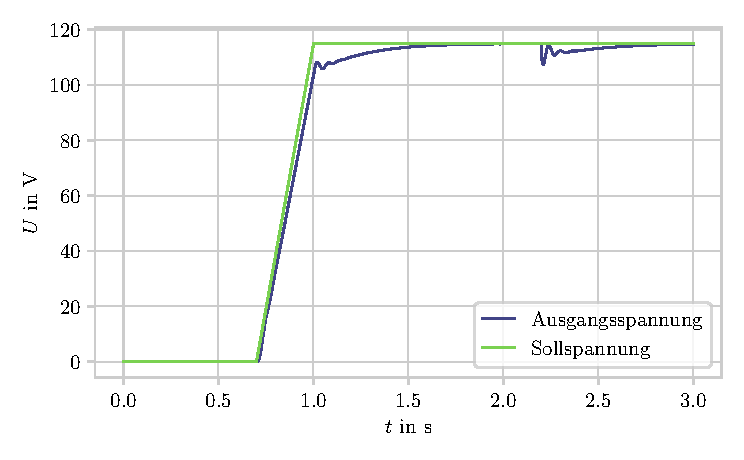
\includegraphics{Bilder/Verifikation_Spannung.pdf}
    \caption{Effektivwert der Ausgangsspannung (LN-Spannung) und Sollwert des Reglers}
    \label{fig:Verifikation_Spannung}
\end{figure}

Die Frequenz der Ausgangsspannung wird im Modell aus Geschwindigkeitsgründen aus der Winkelgeschwindigkeit der Welle und der Polpaarzahl des Synchrongenerators ermittelt. Um die Kopplung der Spannungsfrequenz mit der Winkelgeschwindigkeit der Welle zu überprüfen, wird die so ermittelte Frequenz mit der Frequenz der Zeitverläufe der drei Phasen der Ausgangsspannung verglichen. \cref{fig:Verifikation_Frequenz} zeigt den Verlauf der Frequenz, ermittelt durch Messen der Zeit zwischen den Nulldurchgängen (blaue Kurve) und die zum gleichen Zeitpunkt aus der Winkelgeschwindigkeit ermittelte Frequenz. Wie zu sehen ist, stimmen beide Kurven miteinander überein. Der Abweichung der Frequenz aus den Nulldurchgängen im Sprungmoment von der Frequenz aus der Winkelgeschwindigkeit erklärt sich aus Abweichungen der Spannung von der reinen Sinusform (Oberschwingungen) im Sprungmoment.
\begin{figure}
    \centering
    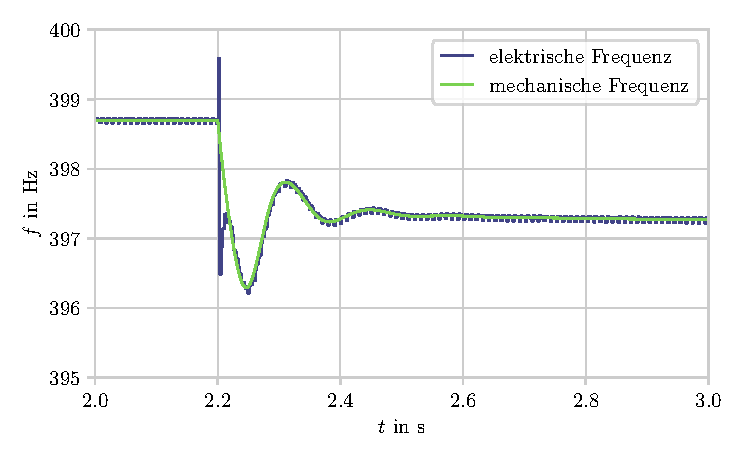
\includegraphics{Bilder/Verifikation_Frequenz.pdf}
    \caption{Frequenz der Ausgangsspannung, ermittelt aus der Zeit zwischen Nulldurchgängen und aus der Winkelgeschwindigkeit}
    \label{fig:Verifikation_Frequenz}
\end{figure}

Schließlich kann die Struktur des Modells und der Verbindungen mittels des Energiefluss zwischen den Teilmodellen überprüft werden. Die Übersicht in \cref{fig:Wirkungsgraph} gibt dazu die Referenz. \cref{fig:VerifikationLeistungen} zeigt Zeitverläufe verschiedener Leistungen an verschiedenen Punkten im Modell. Aus der Netzspannungsquelle wird elektrische Leistung vom Stator der Asynchronmaschine über den Luftspalt auf die Welle übertragen. Die Differenz zwischen den Leistungen ergibt sich aus den elektrischen Verlusten im Stator und im Rotor und aus den Verlusten im Luftspalt. Die mechanische Leistung teilt sich auf den Synchrongenerator und die Erregermaschine auf, wobei der Hauptteil von dem Generator aufgenommen wird. Die Erregemaschine erhält neben der mechanischen Leistung einen kleinen Beitrag aus der Erregung durch den Spannungsregler und giibt die erzeugte elektrische Leistung an den Synchrongenerator als Erregung ab. Der Synchrongenerator erzeugt dann aus der mechanischen Leistung elektrische Energie (ebenfalls verlustbehaftet), die an den Ausgang abgegeben wird. Mit Berücksichtigung der Verlustleistungen stimmen die Kurven miteinander überein, wobei beachtet werden muss, dass die Abweichungen im Sprungmoment von der Aufnahme oder Abgabe von Energie aus Speichern wie der rotatorischen Trägheit verursacht wird.
\begin{figure}
    \centering
    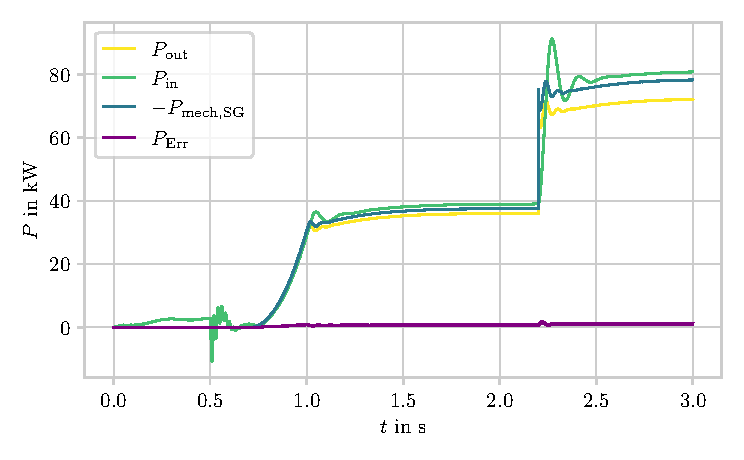
\includegraphics{Bilder/Verifikation_Leistung.pdf}
    \caption{Übersicht über die übertragenen Leistungen}
    \label{fig:VerifikationLeistungen}
\end{figure}

Damit können die wichtigsten Eigenschaften des Modells als plausibel betrachtet werden. Im nächsten Schritt wird dann untersucht, wie das Modell mit dem realen Umformer übereinstimmt.

\section{Validierung}
\label{sec:Validierung}
Die Validierung des Simulationsmodells hat zum Ziel Übereinstimmung zwischen dem realen Verhalten der Anlage und dem Verhalten des Modells zu gewährleisten. Dabei muss berücksichtigt werden, dass jedes Übereinstimmen nur in bestimmten Grenzen möglich sein kann, da jedes Modell eine Vereinfachung der Realität darstellt. Die Validierung erfolgt durch Vergleich des Modellverhaltens mit den in \cref{chap:Versuch} aufgenommenen und aufbereiteten Messdaten. 

Das begründet eine zusätzliche Einschränkung der Möglichkeiten zur Validierung des Modells, da zum Einen jede Messung fehlerbehaftet ist und zum Anderen nur beschränkte Möglichkeiten zur Messung des Systems zur Verfügung standen. So war es nur möglich, die Polradspannung und die elektrischen Ein- und Ausgangsgrößen des Systems aufzunehmen. Messung der Zeitkonstanten oder Induktivitäten der elektrischen Maschinen konnten an der betrachteten Anlage nicht ohne erheblichen Aufwand durchgeführt werden, da die elektrischen Maschinen nicht einzeln zugänglich waren.

\paragraph{Drehzahl-Drehmoment-Kennlinie der ASM}
Die Drehzahl-Drehmoment-Kennlinie des Asynchronmotors beeinflusst das Verhalten der elektrischen Anlage bei Belastung: Je steiler (\emph{härter}) die Kennlinie des Motors ist, desto weniger stark wird der Motor verlangsamt durch Erhöhung des Lastmoments. Die Frequenz der Ausgangsspannung ändert sich also weniger bei Belastung der Maschine. Aus den Messdaten kann die Kennlinie mit Hilfe der Ein- und Ausgangsleistungen und der Frequenz der Ausgangsspannung gewonnen werden. Die Winkelgeschwindigkeit der Welle ist nach \cref{eq:Winkelgeschwindigkeit-Frequenz} 
\begin{equation}
    \omega_{\mathrm{mech}} = \frac{2\pi}{f_{\mathrm{out}}} \label{eq:Winkelgeschwindigkeit-Frequenz}
\end{equation}
über die Polpaarzahl mit der Spannungsfrequenz verknüpft. Mit Kenntnis der Winkelgeschwindigkeit kann das maximale bzw. minimale Drehmoment, das über die Welle übertragen wird, aus den Leistungen nach \cref{eq:Moment-ASM} bestimmt werden.
\begin{equation}
    \frac{P_{\mathrm{out}} - P_{\mathrm{Regler}}}{\omega_{\mathrm{mech}}} < M_{\mathrm{ASM}} < \frac{P_{\mathrm{in}}}{\omega_{\mathrm{mech}}} \label{eq:Moment-ASM}
\end{equation}

Die Kennlinie des Simulationsmodells der ASM wird mit Hilfe einer separaten Simulation erzeugt. Die Winkelgeschwindigkeit der ASM wird über eine Rampenfunktion vorgegeben. Über einen Zeitraum von $\unit[10]{s}$ wird die Winkelgeschwindigkeit von $\omega_{\mathrm{mech}}=\unit[305]{\frac{rad}{s}}$ auf $\unit[315]{\frac{rad}{s}}$ erhöht (das entspricht dem Arbeitsbereich der ASM), sodass die Änderungen quasi-stationär stattfinden.
Damit ergibt sich die Drehzahl-Drehmoment-Kennlinie der ASM in \cref{fig:Validierung-ASMKennlinie}. Das Anpassen der simulierten Kennlinie an die Messdaten erfolgte durch Einstellen des Rotorwiderstands der ASM. Auch ein Abgleich anderer Größen der ASM wäre möglich gewesen. Jedoch lässt sich die Änderung der Kennlinie dann nicht eindeutig einer einzigen Variablen zuordnen, wodurch die Komplexität dieses Einstellverfahrens deutlich erhöht wird.
\begin{figure}
    \centering
    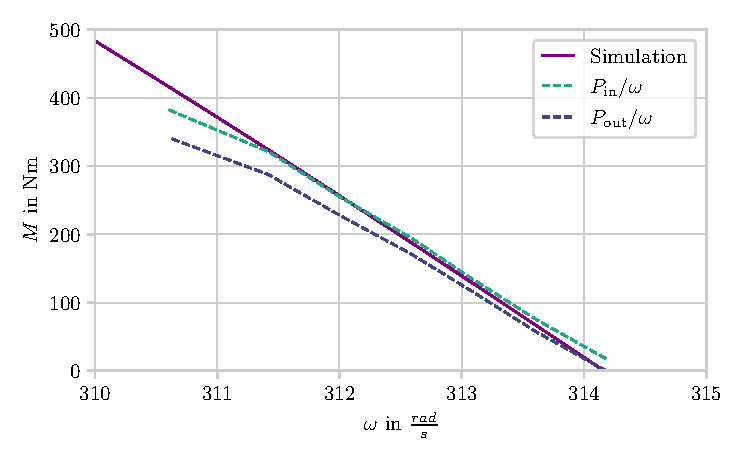
\includegraphics{Bilder/Validierung_Kennlinie.pdf}
    \caption{Drehzahl-Drehmomentkennlinie der Asynchronmaschine aus der Simulation und der Messung}
    \label{fig:Validierung-ASMKennlinie}
\end{figure}

\paragraph{Spannungskennlinie der Erregermaschine}
\begin{figure}[h!]
    \centering
    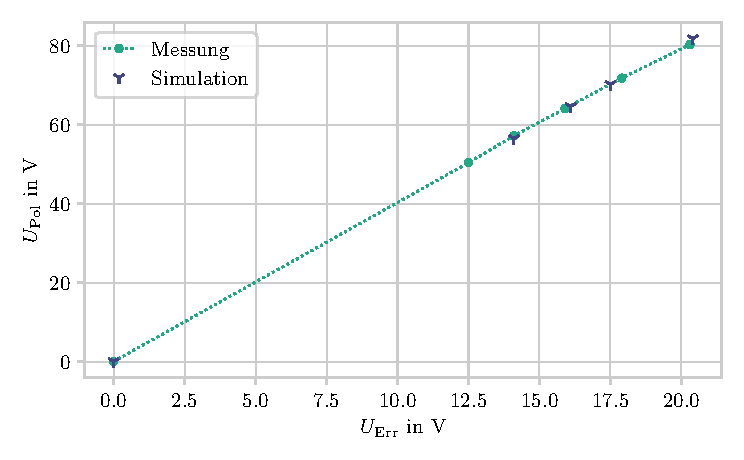
\includegraphics{Bilder/Validierung_Erregermaschine.pdf}
    \caption{Spannungkennlinie der Erregermaschine}
    \label{fig:Validierung-Erregermaschine}
\end{figure}
Die Spannungskennlinie der Erregermaschine beschreibt den Zusammenhang zwischen der Stellgröße des Reglers (der Erregerspannung) und der damit eingestellten gleichgerichteten Polradspannung zur Erregung des Synchrongenerators. Über die Impedanz des Synchrongenerators stellt sich durch die Polradspannung der Erregerstrom ein, der bei der hier betrachteten Maschine über die Schleifringe nicht gemessen werden konnte. Der Abgleich der Spannungskennlinie mit den Messdaten erfolgte durch Aufbringen verschiedener Lastsprünge in der Simulation und anpassen der Erregerwiderstände der Erregermaschine und des Synchrongenerators. Die resultierende Spannungskennlinie zeigt \cref{fig:Validierung-Erregermaschine}.

\paragraph{Verschiedene Lastsprünge}
Die Simulationsergebnisse des angepassten Modells werden mit der Messung verglichen. Betrachtet wird die Ausgangsspannung bei Ausführen verschiedener Lastsprünge mit $cos(\varphi)=0,8$. Dieser Leistungsfaktor wird gewählt, da hier die Spannungsamplituden im Sprungmoment größer sind (vgl. \cref{fig:ZeitverlaufDynamischOhneRegleraenderung}). Aus dem Vergleich der Simulationseregbnisse mit den Messergebnissen kann der Modellierungsfehler bestimmt werden. Quantifiziert wird der Fehler mit dem mittleren absoluten Fehler (\emph{\textbf{M}ean \textbf{A}bsolute \textbf{E}rror} -- MAE)
\begin{equation}
\mathrm{MAE} = \mathrm{mean}\left(\left| \hat{y} - y \right|\right).
\end{equation}
\Cref{fig:Spannung} zeigen die gemessenen und simulierten Spannungen bei verschiedenen Lastsprunggrößen. Die simulierten Spannungen stimmen gut mit den Messungen ein. Der schlecteste MAE beträgt 0,6. Weiterhin zeigt sich, dass die kleineren Lastsprünge auch mit einem kleineren Fehler behaftet sind. Der kleinste Fehler tritt im Lastbereich von \unit[50]{\%} bis \unit[100]{\%} auf.
\begin{figure}
\centering
\begin{subfigure}{.49\textwidth}
	\centering
	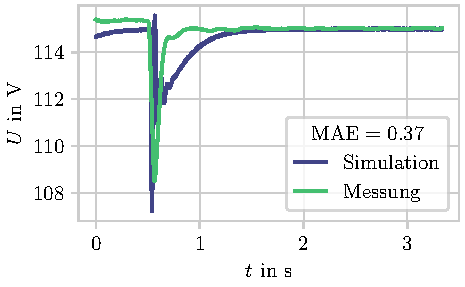
\includegraphics[]{Bilder/ValMessung_0-50.pdf}
	\caption{Lastsprung \unit[0]{\%}-\unit[50]{\%}}
	\label{fig:ValMessung0-50}
\end{subfigure}
\begin{subfigure}{.49\textwidth}
	\centering
	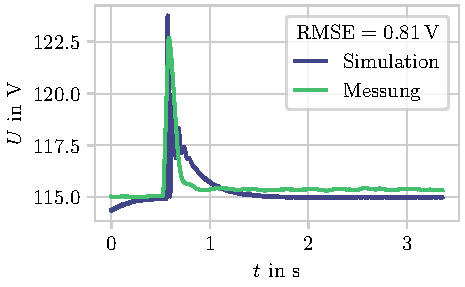
\includegraphics[]{Bilder/ValMessung_50-0.pdf}
	\caption{Lastsprung \unit[50]{\%}-\unit[0]{\%}}
	\label{fig:ValMessung50-0}
\end{subfigure}
\begin{subfigure}{.49\textwidth}
	\centering
	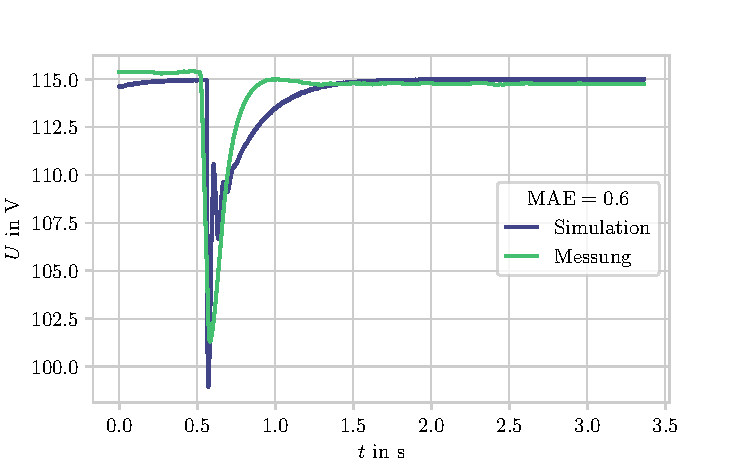
\includegraphics[]{Bilder/ValMessung_0-100.pdf}
	\caption{Lastsprung \unit[0]{\%}-\unit[100]{\%}}
	\label{fig:ValMessung0-100}
\end{subfigure}
\begin{subfigure}{.49\textwidth}
	\centering
	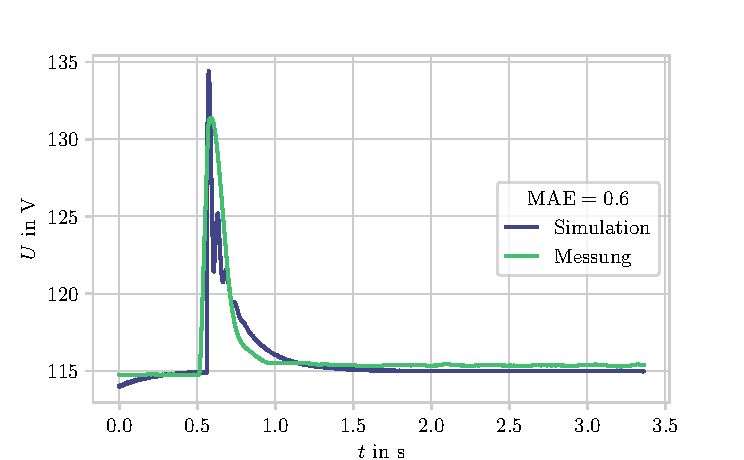
\includegraphics[]{Bilder/ValMessung_100-0.pdf}
	\caption{Lastsprung \unit[100]{\%}-\unit[0]{\%}}
	\label{fig:ValMessung100-0}
\end{subfigure}
\begin{subfigure}{.49\textwidth}
	\centering
	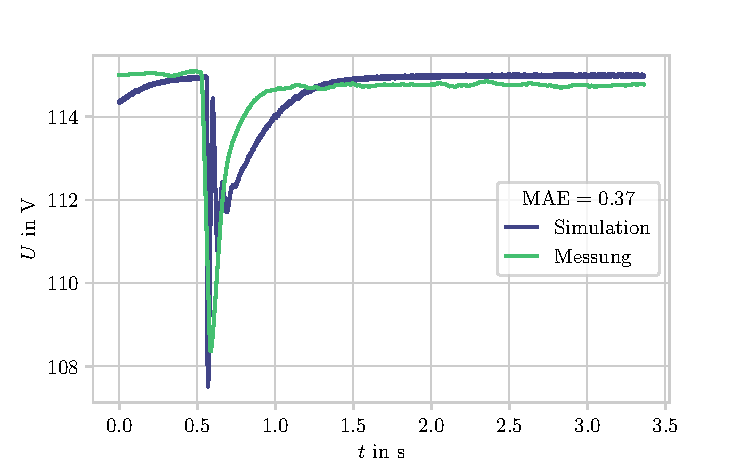
\includegraphics[]{Bilder/ValMessung_50-100.pdf}
	\caption{Lastsprung \unit[50]{\%}-\unit[100]{\%}}
	\label{fig:ValMessung50-100}
\end{subfigure}
\begin{subfigure}{.49\textwidth}
	\centering
	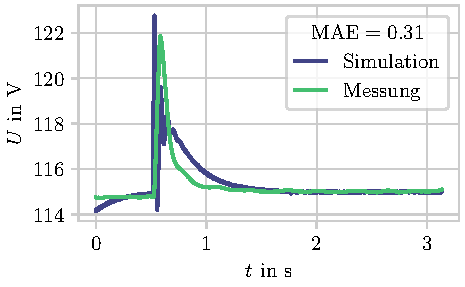
\includegraphics[]{Bilder/ValMessung_100-50.pdf}
	\caption{Lastsprung \unit[100]{\%}-\unit[50]{\%}}
	\label{fig:ValMessung100-50}
\end{subfigure}
\caption{Gemessene und simulierte Ausgangsspannungen bei verschiedenen Lastsprüngen}
\label{fig:ValSpannung}
\end{figure}